\begin{center}
{\Large\bfseries\reporttitle\par}
\vspace{0.35em}
{\normalsize Revathi Eedala Venkatesulu, Jean-Pierre Tas, Chi Kien Ngo, Sahiti Vuyyuru\par}
{\small California State University, Long Beach\par}
\end{center}

\begin{abstract}
Large language models can generate continuous integration configurations, but evaluating their usefulness requires more than textual similarity. This study replicates the statistical analysis of a 2025 GitHub Actions study and extends it using 1,318 examples and 7,908 archived model outputs. We independently calculate lexical and path--value agreement, examine repeated documentation tasks, and evaluate candidate selection with parsing and a pinned static workflow checker. GPT-4o has the highest archived row-weighted mean cosine similarity, 0.688, but its paired difference from GPT-4.1 is not statistically significant. Equal weighting of source pages reverses their ranking. Consensus selection raises path--value F1 from 0.259 to 0.283 relative to syntax-only fallback; the gain persists when root-kind credit is removed, while lexical agreement decreases. On 335 examples shaped as complete workflows, checker-guided fallback accepts 284 candidates, compared with 264 for the strongest individual model, an increase of 5.97 percentage points; 51 cases receive explicit abstention. This coverage gain persists under task-pair and source-page weighting, and five candidates reach the full six-candidate coverage. A reference-integrity audit identifies preprocessing damage and perfect tree scores caused by two parsing failures. Functional correctness requires execution-based evidence and was not evaluated here.
\end{abstract}
\noindent\textbf{Keywords:} generative AI; software engineering; continuous integration; GitHub Actions; replication; YAML validation.

\section{Introduction}
A GitHub Actions configuration can pass a generic parser and still lack the trigger that starts the workflow. It can also resemble a reference closely while using an obsolete action or omitting a required step. These failures make continuous integration (CI), which automates building and testing around repository changes, a concrete test of how large language model (LLM) outputs should be evaluated. Fan et al. identify the integration of LLMs with established software engineering methods as an open research problem~\cite{fan2023}. Here, the immediate question is what evidence a generated configuration must pass before its similarity score becomes useful.

GitHub Actions represents automation using YAML Ain't Markup Language (YAML) documents. Workflow behavior depends on configuration structure and the surrounding repository. Mastropaolo et al. study completion of existing workflow configurations, whereas Zhang et al. evaluate several workflow-related tasks with different prompting conditions~\cite{mastropaolo2024,zhang2024}. Their task definitions and datasets differ from generation from documentation descriptions; their reported success rates therefore answer different questions.

The selected replication article, by Ghaleb and Rathnayake, evaluates six models on 1,318 description--YAML examples extracted from GitHub Actions documentation~\cite{ghaleb2025}. It reports approximately 0.69 mean cosine similarity for GPT-4o and only about 3\% perfect matches. Our inspection of the released data raises two issues behind that contrast: the 1,318 rows contain only 690 distinct description--reference pairs, and the tree-scoring implementation can assign perfect similarity when both inputs fail to parse. Repeating the model ranking alone would leave both issues unresolved.

The replication phase retains the original six models, five archived metrics, and paired statistical comparisons. We then extend that analysis by tracing reference transformations, changing the unit of aggregation, and selecting among the six archived candidates without consulting the reference answer. This connects each extension to a specific weakness in the original evaluation. We address three research questions (RQs):
\begin{enumerate}[label=\textbf{RQ\arabic*.}]
\item How do the archived results and independently recomputed measures characterize model performance?
\item How do repeated description--reference pairs and source-page weighting affect model comparisons?
\item Can parser-aware and domain-aware candidate selection improve static acceptance and reference agreement among the archived candidates?
\end{enumerate}

All experiments use the supplied historical outputs. The resulting contribution is an audited comparison and an implemented static selector; no new model responses or workflow executions are included. The following methodology defines the measurements and the boundary between those two contributions.

\section{Proposed Methodology}
The analysis separates reproduction of archived measurements from new measurements of the preserved texts. All inputs come from the supplied replication package~\cite{package}. The original files remain unchanged, and every result is joined by example identifier. Appendix~\ref{app:reproducibility} maps the analysis scripts and exported evidence to the results reported below.

\subsection{Replication boundary and metric audit}
We recompute model means and statistical comparisons from the released score table using the original measurement definitions. New lexical and structural agreement measures are calculated from the unchanged documentation references and archived outputs. The original embedding and tree-distance columns remain archived measurements.

Table~\ref{tab:metrics} describes the five released score columns using the implementation rather than relying only on their labels. The original paper describes cosine and Euclidean comparisons using term frequency--inverse document frequency (TF-IDF) vectors. In contrast, the code loads \texttt{all-MiniLM-L6-v2} through Sentence Transformers and encodes each string. That model is an embedding model~\cite{sbert}; its cosine score is not a direct measure of exact token overlap. We therefore refer to the archived quantity as cosine similarity without asserting that it is a TF-IDF score.

\begin{table}[H]
\centering\small
\caption{Operational meaning of the released similarity columns. All are interpreted as similarities, with larger values indicating closer agreement under that implementation.}
\label{tab:metrics}
\begin{tabularx}{\linewidth}{@{}lY@{}}
\toprule
Released column & Implementation and interpretation\\
\midrule
CosineSimilarity & Cosine between sentence-transformer embeddings of comment-cleaned strings.\\
EuclideanDistance & Stored as $1/(1+\lVert u-v\rVert_2)$, so the column contains similarity rather than raw distance.\\
TreeEditDistance & Active function uses $\max(0,\min(1,1-d/(2\max(n_r,n_g))))$ for tree edit distance $d$ and node counts $n_r,n_g$. Parser exceptions return an empty root.\\
ROUGE-L & Recall-Oriented Understudy for Gisting Evaluation using longest common subsequences, but code returns the maximum of precision, recall, and F-score rather than only F-score.\\
chrF & Character n-gram F-score, lowercased with whitespace retained; stored on a 0--1 scale.\\
\bottomrule
\end{tabularx}
\end{table}

Two tree-similarity functions share a name; Python uses the second definition. The prompt script combines title and description, although the displayed paper prompt presents a description field. It also saves reference strings using \texttt{strip()}, while its output filenames differ from those expected by the analysis script.

\subsection{Independent raw-text and structural measurements}
The new measurements use raw documentation references and raw archived responses, preserving indentation and comments. We calculate the F1 form of Recall-Oriented Understudy for Gisting Evaluation using longest common subsequences (ROUGE-L) over whitespace-delimited tokens~\cite{lin2004}. For longest common subsequence length $L$ and token counts $n_r,n_g$, the score is $2L/(n_r+n_g)$, with zero assigned to an empty sequence. We also calculate the character n-gram F-score (chrF)~\cite{popovic2015} with SacreBLEU 2.5.1~\cite{sacrebleu}: character orders 1--6, no word n-grams, $\beta=2$, case preserved, whitespace excluded, effective-order handling, and epsilon smoothing disabled. A separate raw-text maximum-of-precision/recall calculation isolates the original ROUGE aggregation choice. These new variants differ from the released preprocessing and cannot be compared as if only the model had changed.

For structural agreement, a string-preserving BaseLoader composition represents each scalar by its exact decoded value and its tuple of mapping keys and sequence indices. Scalar node tags, a root-kind feature, and explicit empty-container features preserve structural distinctions. Mapping-key order is ignored; sequence order matters. Duplicate mapping keys, complex keys, cyclic aliases, empty documents, and parsing failures are recorded explicitly. For reference feature set $R$ and generated set $G$, path--value F1 is
\[
 F_{\mathrm{pv}}=\frac{2|R\cap G|}{|R|+|G|}.
\]
Invalid references are excluded from this structural comparison. On the fixed set of valid references, invalid generated candidates receive zero; conditional means over two valid parses are exported separately. A feature-identical configuration is called an exact structural match, which permits formatting changes but does not assert behavioral equivalence. We also repeat scoring without the root-kind feature to check sensitivity to that design choice.

\subsection{Statistical comparison and aggregation}
For RQ1, we calculate each model's mean on all 1,318 rows for all five metrics. We repeat the original two-sided paired Wilcoxon signed-rank comparisons of GPT-4o cosine scores against the five alternatives and apply Holm correction to that family of five tests. We also repeat Spearman correlations between description word count and the four GPT-4o metrics selected by the released correlation function, with a separate Holm correction. The code omits chrF from that function even though the paper describes five metrics. A corrected $p<0.05$ is interpreted as evidence of a distributional difference under the test assumptions, not as proof of practical superiority.

For RQ2, we distinguish three estimands. The row mean weights each released example equally. The pair-balanced mean gives equal weight to each exact description--reference group in the unchanged documentation table: first average model scores within a repeated pair, then average the group means. Keeping all archived outputs within a group avoids arbitrarily selecting the first response. The source-page mean first averages within each source uniform resource locator (URL), then gives each of the 186 source pages equal weight. These quantities answer different questions: expected score for a released row, for a distinct archived task pair, and for a source page.

We additionally estimate uncertainty in the row-weighted GPT-4o minus GPT-4.1 mean cosine difference using a paired source-URL cluster bootstrap. Each of 10,000 resamples draws 186 URLs with replacement and retains all rows belonging to each sampled URL, including multiplicities. We recompute the row-weighted difference and report percentile 95\% intervals with random seed 2026. This preserves model pairing and within-page dependence, but does not eliminate dependence from duplicated examples appearing on different pages. Bootstrap intervals describe this dataset and sampling convention, not a population of all software repositories.

\subsection{Parser-aware evaluation and candidate selection}
For RQ3, we use two explicit loading policies~\cite{pyyaml}. \texttt{SafeLoader} reproduces the loading behavior used in the original tree function. \texttt{BaseLoader} supplies a separate syntax-oriented check that avoids implicit Boolean conversion of keys such as \texttt{on}. BaseLoader checks whether the text can be loaded, but does not validate the GitHub Actions schema, unique mapping keys, expression semantics, or command behavior. Empty documents are rejected by the candidate-selection rule. YAML's representation and typing rules must be distinguished from the domain rules of a workflow~\cite{yaml}.

The audit loads the original documentation reference, the reference saved with each model output, and the common reference field retained in the merged score table. These texts are checked separately because the supplied files are not fully synchronized. We apply the released comment-removal function exactly when investigating the original failure path. For tree-score interpretation, each pair receives an explicit reference/output loading status. If either fails, structural similarity is treated as unavailable in the parser-aware view; it is not replaced with a fabricated empty tree.

The fixed candidate priority is GPT-4o, GPT-4.1, Gemma3, Llama3.1, CodeGemma, and Code Llama. We compare four reference-free selectors: syntax fallback selects the first nonempty BaseLoader candidate; strict fallback additionally rejects the structural error states above; consensus selects the strict candidate with the highest mean pairwise path--value F1 to the other eligible candidates; and minimal structure selects the strict candidate with the fewest features. Ties follow the fixed priority. The consensus and minimality rules test whether agreement among candidates or restraint in adding structure improves reference agreement. Neither rule sees the reference answer.

All policies are evaluated on the same tasks, retaining abstentions as zero candidate agreement on valid references. Policy differences use paired URL-cluster percentile intervals with 10,000 resamples and seed 2026. The comparison is exploratory: no selector is tuned on a held-out dataset, and improved reference agreement is not interpreted as improved functional correctness.

\subsection{Static workflow validation and domain-aware fallback}
Domain validation is restricted to a task scope defined before checker execution: the raw reference must load as a mapping with an \texttt{on} key and a mapping-valued \texttt{jobs} field. The rule identifies complete-workflow-shaped examples, not proven correct workflows. Other snippets and action-definition-shaped mappings are reported separately. Every reference and all six candidates in this scope are checked, and a second stratum contains the references that themselves pass the checker.

We run actionlint 1.7.7, released January 19, 2025, to check workflow structure, expressions, action usage, and related static constraints~\cite{actionlint}. Its official release archive is verified against the published checksum. Text is passed unchanged through standard input in a neutral temporary directory, with ShellCheck and Pyflakes integrations disabled. No repository-specific configuration, companion workflow files, or generated commands are executed. Acceptance means exit status zero under this configuration. Local action paths and reusable-workflow references are flagged because their repository context is unavailable.

Domain-aware fallback applies the same candidate priority but selects the first checker-accepted candidate, abstaining if all six are rejected. References determine the retrospective task stratum, never which candidate is chosen. We report checker acceptance over every task in the stratum, accepted-candidate counts, abstentions, and exact reference agreement. The candidate-selection interface requires an explicitly declared fragment or workflow scope.

For a further sensitivity analysis, we recalculate workflow acceptance with equal weight per exact task pair and per source page. We estimate the paired fallback-minus-GPT-4.1 coverage difference with the same cluster-bootstrap procedure, restricted to URLs represented in the workflow stratum. We also evaluate successive prefixes of the fixed candidate order, from one to six candidates. These prefixes measure the contribution of each archived candidate; they do not estimate the cost or quality of repeated sampling from one model.

\section{Case Study and Data Preparation}
The selected International Conference on Software Maintenance and Evolution (ICSME) article provides a documentation-derived GitHub Actions benchmark. The local release contains the documentation table, six archived model-output files, a combined similarity table, and scripts for collection, prompting, and scoring. It includes GPT-4o, GPT-4.1, Llama3.1--8B, Gemma3--12B, Code Llama--7B, and CodeGemma--7B. We retain the release's model labels and do not generalize from them to all general-purpose or code-specialized models.

All seven input tables and the combined score table contain the same 1,318 unique identifiers. We align by identifier rather than relying on incidental row order and verify that paired comparisons have complete observations. Source addresses are treated as historical provenance fields, not fetched again to replace the benchmark with today's documentation. The analysis exports input Secure Hash Algorithm 256-bit (SHA-256) hashes and dependency versions so the supplied snapshot remains identifiable.

\begin{table}[H]
\centering\small
\caption{Profile of the supplied documentation benchmark and its archived scores.}
\label{tab:data}
\begin{tabular}{@{}lr@{}}
\toprule
Property & Count\\
\midrule
Example identifiers & 1,318\\
Archived model outputs & 7,908\\
Distinct raw description--reference pairs & 690\\
Repeated pair rows beyond one per group & 628\\
Distinct raw reference strings & 603\\
Distinct source pages (URLs) & 186\\
Distinct pairs in transformed score table & 691\\
\bottomrule
\end{tabular}
\par\vspace{0.3em}{\footnotesize Raw pair grouping uses exact Description and Code fields in the documentation table. The separately transformed score table has a different pair count.}
\end{table}


The 1,318 identifiers do not represent 1,318 independent tasks: descriptions and code fragments recur, sometimes under different documentation pages (Table~\ref{tab:data}). Exact matching is intentionally conservative; it does not identify paraphrases or semantically equivalent YAML. Pair balancing therefore reduces only the most directly observable repetition. This distinction also matters in the workflow subset, where 335 rows correspond to 175 exact task pairs across 127 source pages.

The archived references also contain discrepancies beyond indentation: the GPT-4o file has five reference cells containing \texttt{\#NAME?} instead of the documentation text (identifiers 350, 475, 851, 1121, and 1122), while GPT-4.1 has two (350 and 851). The common reference column in the score table differs from the cleaned GPT-4o cached reference at six identifiers. We do not infer how these discrepancies arose. Raw documentation pairs are therefore used for grouping, and per-model cached references are used when checking the original parser failure path.

The dataset mixes complete-workflow-shaped examples with partial mappings, step lists, scalar examples, and action definitions. The predefined scope classification yields 335 workflow-shaped references, 814 mapping fragments, 83 sequence fragments, 54 action-definition-shaped mappings containing a \texttt{runs} key, 24 parse failures, and eight scalar or empty examples. Thus, only about one quarter of the examples enter full-workflow static validation. GitHub's workflow syntax describes a domain-specific document containing triggers and jobs~\cite{githubsyntax}, but documentation often explains one field at a time. We consequently avoid calling every loadable item a valid workflow or every fragment lacking a trigger defective. For path--value scoring, 1,293 references are structurally eligible; the 24 parse failures and one empty document are excluded. Lexical metrics still use all 1,318 texts.

\section{Results and Discussion}
The results follow the three research questions: first the reproduced comparisons and new agreement measures, then weighting sensitivity, and finally reference diagnostics and candidate selection. A model's position is interpreted within each measurement and task scope.

\subsection{RQ1: Reanalysis of the released results}
\begin{table}[H]
\centering\small
\caption{Recomputed means of the released score columns; 1,318 observations per model.}
\label{tab:scores}
\begin{tabular}{@{}lrrrrr@{}}
\toprule
Model & Cosine & Euclidean sim. & Tree sim. & ROUGE-L & chrF\\
\midrule
GPT-4o & 0.688 & 0.589 & 0.663 & 0.562 & 0.508\\
GPT-4.1 & 0.681 & 0.576 & 0.641 & 0.564 & 0.499\\
Gemma3--12B & 0.652 & 0.572 & 0.647 & 0.507 & 0.423\\
Llama3.1--8B & 0.648 & 0.564 & 0.629 & 0.488 & 0.437\\
CodeGemma--7B & 0.639 & 0.563 & 0.621 & 0.469 & 0.418\\
Code Llama--7B & 0.611 & 0.545 & 0.609 & 0.474 & 0.416\\
\bottomrule
\end{tabular}
\par\vspace{0.3em}{\footnotesize Similarity scores are reused from the release; summaries are newly computed. Tree scores retain the original parser failure behavior.}
\end{table}


GPT-4o has the highest mean cosine similarity at approximately 0.688, with GPT-4.1 close behind at approximately 0.681 (Table~\ref{tab:scores}). Code Llama has the lowest mean cosine similarity. These measurements agree with the original rounded cosine values.

\begin{table}[H]
\centering\small
\caption{Two-sided paired Wilcoxon tests: GPT-4o cosine scores versus each alternative; Holm family of five comparisons.}
\label{tab:wilcoxon}
\begin{tabular}{@{}lrrr@{}}
\toprule
Alternative & Mean difference & Raw $p$ & Adjusted $p$\\
\midrule
GPT-4.1 & +0.0069 & $0.430$ & $0.430$\\
Gemma3--12B & +0.0356 & $2.99\times 10^{-23}$ & $5.98\times 10^{-23}$\\
Llama3.1--8B & +0.0394 & $1.46\times 10^{-24}$ & $4.39\times 10^{-24}$\\
CodeGemma--7B & +0.0486 & $1.39\times 10^{-29}$ & $5.58\times 10^{-29}$\\
Code Llama--7B & +0.0762 & $6.20\times 10^{-56}$ & $3.10\times 10^{-55}$\\
\bottomrule
\end{tabular}
\par\vspace{0.3em}{\footnotesize All comparisons contain 1,318 pairs; zero differences are excluded from signed-rank computation. Positive differences favor GPT-4o.}
\end{table}


GPT-4o differs significantly from the four smaller open models in this row-level comparison, but the comparison with GPT-4.1 has corrected $p=0.430$ (Table~\ref{tab:wilcoxon}). The highest mean therefore supports a descriptive ranking, while this test does not establish GPT-4o's superiority over GPT-4.1. Failure to reject a difference is also not an equivalence result. A practical equivalence claim would require an explicit tolerance and a suitable analysis.

\begin{table}[H]
\centering\small
\caption{Spearman correlation of description word count with GPT-4o scores; 1,318 rows and the original four-test Holm family.}
\label{tab:correlation}
\begin{tabular}{@{}lrr@{}}
\toprule
Metric & $\rho$ & Adjusted $p$\\
\midrule
Cosine & 0.198 & $1.52\times 10^{-12}$\\
Euclidean similarity & 0.198 & $1.52\times 10^{-12}$\\
Tree similarity & 0.118 & $1.87\times 10^{-5}$\\
ROUGE-L & 0.187 & $1.56\times 10^{-11}$\\
\bottomrule
\end{tabular}
\end{table}


\begin{samepage}
Longer descriptions are weakly associated with higher archived scores (Table~\ref{tab:correlation}), but correlation does not show that lengthening a prompt would improve the resulting workflow. Task complexity, repetition, and documentation style may all influence the relationship. The reproduced tests use rows as paired observations, as the original implementation does.
\par\end{samepage}

\begin{table}[H]
\centering\small
\caption{Independently recomputed agreement and reference-free selection results.}
\label{tab:rawmetrics}
\begin{tabular}{@{}lrrrrr@{}}
\toprule
Model or selector & ROUGE F1 & chrF & $F_{\mathrm{pv}}$ & Leaf F1 & Exact structure\\
\midrule
GPT-4o & 0.366 & 0.455 & 0.255 & 0.115 & 37\\
GPT-4.1 & 0.330 & 0.449 & 0.242 & 0.116 & 4\\
Gemma3--12B & 0.320 & 0.372 & 0.257 & 0.084 & 34\\
Llama3.1--8B & 0.292 & 0.383 & 0.216 & 0.074 & 21\\
CodeGemma--7B & 0.278 & 0.366 & 0.216 & 0.076 & 25\\
Code Llama--7B & 0.257 & 0.368 & 0.184 & 0.058 & 2\\
Syntax fallback & 0.366 & 0.456 & 0.259 & 0.116 & 37\\
Strict fallback & 0.368 & 0.456 & 0.261 & 0.117 & 37\\
Consensus & 0.340 & 0.406 & 0.283 & 0.127 & 48\\
Minimal structure & 0.349 & 0.380 & 0.291 & 0.102 & 51\\
\bottomrule
\end{tabular}
\par\vspace{0.3em}{\footnotesize Lexical means use 1,318 examples. Structural means and exact counts use the same 1,293 valid references, assigning zero to invalid generated candidates. Leaf F1 removes the shared root-kind feature. Selectors use only candidate text.}
\end{table}


GPT-4o has the highest raw ROUGE F1, 0.366, and chrF, 0.455 (Table~\ref{tab:rawmetrics}). Structural rankings depend on representation: Gemma3 leads the root-augmented path--value measure at 0.257, while GPT-4.1 and GPT-4o are close on the leaf-only variant at approximately 0.116 and 0.115. The values describe reference overlap rather than a percentage of correct workflows.

For GPT-4o, the archived maximum-style score is 0.562; recalculating maximum precision/recall/F1 on raw text gives 0.555, and changing only that aggregation to F1 gives 0.366. For GPT-4.1, the corresponding values are 0.564, 0.539, and 0.330. This isolates a substantial formula effect on identical raw inputs; the remaining difference combines reference, preprocessing, and artifact-version effects. It should not be interpreted as a change in the models themselves.

On the 335 workflow-shaped references, GPT-4.1 has higher raw ROUGE F1 than GPT-4o, 0.435 versus 0.367, and higher leaf agreement, 0.149 versus 0.084.

\subsection{RQ2: Sensitivity to repeated examples and source pages}
\begin{table}[H]
\centering\small
\caption{Cosine means under alternative aggregation units.}
\label{tab:aggregation}
\begin{tabular}{@{}lrrr@{}}
\toprule
Model & 1,318 rows & 690 raw task pairs & 186 source pages\\
\midrule
GPT-4o & 0.688 & 0.676 & 0.686\\
GPT-4.1 & 0.681 & 0.670 & 0.706\\
Gemma3--12B & 0.652 & 0.638 & 0.664\\
Llama3.1--8B & 0.648 & 0.643 & 0.656\\
CodeGemma--7B & 0.639 & 0.631 & 0.660\\
Code Llama--7B & 0.611 & 0.610 & 0.646\\
\bottomrule
\end{tabular}
\par\vspace{0.3em}{\footnotesize Pair means average all archived responses within each exact raw documentation pair before giving each pair equal weight. Page means give each URL equal weight.}
\end{table}


Pair balancing lowers GPT-4o's mean from 0.688 to 0.676 and places Llama3.1 above Gemma3, reversing their row-level order (Table~\ref{tab:aggregation}). Giving each source page equal weight produces a larger change at the top: GPT-4.1 scores 0.706 and GPT-4o 0.686.

\begin{figure}[H]
\centering
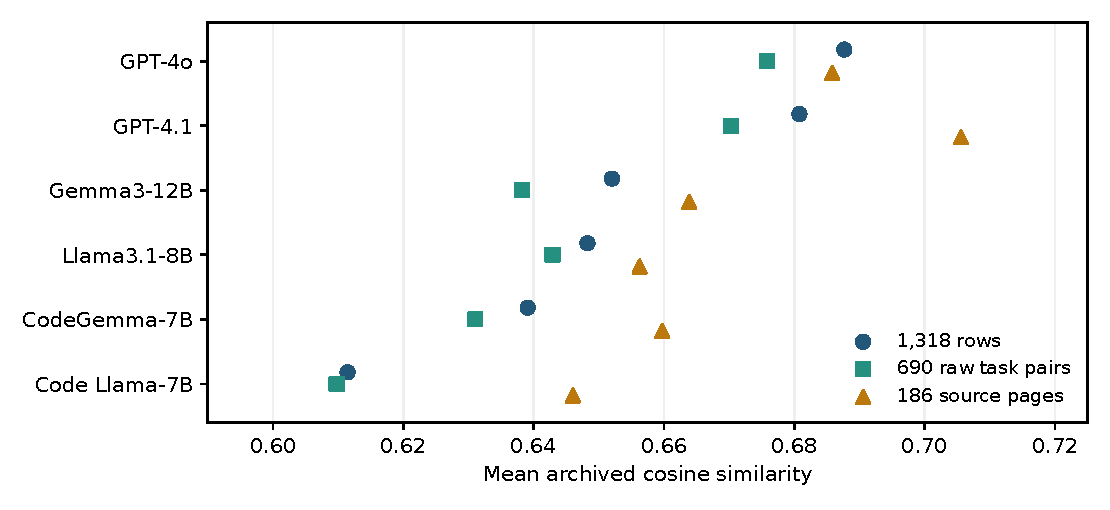
\includegraphics[width=\linewidth]{figures/aggregation.pdf}
\caption{Cosine similarity under row, description--reference pair, and source-page weighting. The unit of aggregation changes the relative position of models, especially the GPT-4o/GPT-4.1 comparison.}
\label{fig:aggregation}
\end{figure}

Figure~\ref{fig:aggregation} compares model scores under row, task-pair, and source-page weighting. Neither aggregation estimates success on a new repository without assumptions about how that repository's tasks resemble the benchmark.

The paired URL-cluster bootstrap gives a row-weighted GPT-4o minus GPT-4.1 mean cosine difference of \CosineDifference{}, with a 95\% percentile interval of \ClusterInterval{}. The interval includes zero.

\subsection{RQ3: Candidate selection and validation}
\subsubsection{Reference integrity before candidate comparison}
The parser audit checks whether the reference and candidate can support a structural comparison before their scores are used to assess selection.
\begin{table}[H]
\centering\small
\caption{Raw-text loading results out of 1,318 examples; loaders and nonempty acceptance are kept distinct.}
\label{tab:parser}
\begin{tabular}{@{}lrrr@{}}
\toprule
Text source & SafeLoader loads & SafeLoader errors & BaseLoader accepts\\
\midrule
Raw documentation reference & 1294 & 24 & 1293\\
GPT-4o & 1281 & 37 & 1281\\
GPT-4.1 & 1277 & 41 & 1277\\
Gemma3--12B & 1276 & 42 & 1276\\
Llama3.1--8B & 1262 & 56 & 1264\\
CodeGemma--7B & 1274 & 44 & 1280\\
Code Llama--7B & 1312 & 6 & 1312\\
\bottomrule
\end{tabular}
\par\vspace{0.3em}{\footnotesize BaseLoader acceptance additionally excludes empty documents. These counts are parser outcomes, not GitHub Actions validity rates.}
\end{table}


Under SafeLoader, 1,294 of 1,318 original documentation references load successfully (Table~\ref{tab:parser}). Applying \texttt{strip()} to those strings reduces this to 1,256. After the original comment-removal operation, the corresponding counts are 1,296 and 1,258. Thus, 38 references that load after comment removal cease to load when the preceding \texttt{strip()} is introduced. This transformation can remove indentation before the first line while leaving subsequent lines unchanged.

An illustrative case is identifier 82, an upload-artifact step list. Its original reference begins with an indented sequence item. Saving the string with \texttt{strip()} removes only the initial indentation of that item, changing its relationship to later lines. The Gemma3 output and the scored reference both fail the original parser, yet their released tree-similarity score is 1.0. In the active tree function, both exceptions become the same empty root, yielding zero edit distance. Identifiers 92 for Code Llama and 74 for Llama3.1 expose the same failure mechanism. Appendix~\ref{app:cases} preserves the reference strings for identifier 82 so the indentation change can be inspected directly.

Across the six models, the audit identifies \FalsePerfectCount{} published perfect tree scores associated with two SafeLoader failures after the original cleaning. These rows are not evidence of perfect structural agreement. The parser-aware extension marks them unavailable and records both error states in the exported table of all 7,908 model--reference pairs; validly loaded pairs retain their archived tree score. The audit also preserves raw text: the original regular expression for inline comment removal can affect hash characters inside quoted values, so its output should not silently replace the original configuration in a validity assessment.

These parsing failures affect particular observations and do not show that parser errors explain the six-model ranking. Parser coercion and tree overlap do not establish identical workflow behavior.

\subsubsection{Structural gains and tradeoffs}
Table~\ref{tab:fallback} shows that syntax-only fallback raises nonempty parser acceptance from 1,281 to 1,318 cases, recovering 37 candidates; exact raw-text agreement remains 16 cases. Relative to Code Llama, the strongest individual model by parser acceptance at 1,312 cases, this adds six accepted cases.

\begin{table}[H]
\centering\small
\caption{Nonempty BaseLoader acceptance for GPT-4o alone and fixed fallback over archived candidates.}
\label{tab:fallback}
\begin{tabular}{@{}lrrrr@{}}
\toprule
Scope & $n$ & GPT-4o & Fallback & Recovered\\
\midrule
All examples & 1318 & 1281 & 1318 & 37\\
Loadable documentation references & 1294 & 1257 & 1294 & 37\\
\bottomrule
\end{tabular}
\par\vspace{0.3em}{\footnotesize The second row uses SafeLoader-loadable raw documentation references. Both policies retain 16 exact matches after outer-whitespace stripping; functional success is unmeasured.}
\end{table}


Consensus raises root-augmented path--value F1 from 0.259 to 0.283 relative to syntax fallback (Table~\ref{tab:rawmetrics}). Removing root-kind credit still gives 0.127 versus 0.116: the paired improvement is 0.0115, with a URL-cluster 95\% interval of [0.0042, 0.0204], using 1,293 fixed reference cases and 184 source pages. Strict fallback alone scores 0.117 on this leaf-only variant; consensus improves on it by 0.0104, with a cluster interval of [0.0030, 0.0192]. The structural gain therefore extends beyond rejecting duplicate keys. Consensus also raises exact structural matches from 37 to 48. Its leaf-only improvement persists under equal task-pair weighting, 0.120 versus 0.107, and equal-page weighting, 0.111 versus 0.089.

Consensus lowers raw ROUGE F1 from 0.366 to 0.340 and chrF from 0.456 to 0.406 relative to syntax fallback. The minimal-structure heuristic has the highest root-augmented score, 0.291, but its leaf-only score falls to 0.102. Its apparent improvement depends on rewarding the shared root-kind feature and is therefore not robust to the measurement choice. The root-removal analysis was added as a sensitivity check after inspecting the preliminary structural results; all policies and both representations are retained in the report.

\subsubsection{Domain-aware workflow selection}
\begin{table}[H]
\centering\small
\caption{Static workflow acceptance with actionlint 1.7.7; complete-workflow-shaped task scope.}
\label{tab:workflow}
\begin{tabular}{@{}lrrrr@{}}
\toprule
Model or selector & Accepted & Rate & Abstained & Reference-pass stratum\\
\midrule
GPT-4o & 36/335 & 10.75\% & 0 & 36/292\\
GPT-4.1 & 264/335 & 78.81\% & 0 & 241/292\\
Gemma3--12B & 47/335 & 14.03\% & 0 & 47/292\\
Llama3.1--8B & 50/335 & 14.93\% & 0 & 49/292\\
CodeGemma--7B & 113/335 & 33.73\% & 0 & 108/292\\
Code Llama--7B & 40/335 & 11.94\% & 0 & 40/292\\
Syntax fallback & 43/335 & 12.84\% & 0 & 43/292\\
Checker fallback & 284/335 & 84.78\% & 51 & 260/292\\
\bottomrule
\end{tabular}
\par\vspace{0.3em}{\footnotesize All 335 tasks remain in the main denominator. References themselves pass in 292 cases. The last column uses only that separately defined 292-task stratum. All generated exact-text matches are zero in both strata; acceptance is a static check.}
\end{table}


On the 335 workflow-shaped tasks, references pass actionlint in 292 cases (87.16\%; Table~\ref{tab:workflow}). GPT-4.1 is the strongest individual model under this configuration, passing in 264 cases (78.81\%). Domain-aware fallback selects a checker-accepted output for 284 tasks (84.78\%), an increase of 20 cases or 5.97 percentage points over that baseline. It abstains on the remaining 51 tasks; those tasks remain in the coverage denominator.

The syntax-only policy accepts a YAML candidate on every task but passes actionlint in only 43 cases (12.84\%). Figure~\ref{fig:workflow} shows the same gap for individual models. On the separate stratum whose references pass the checker, domain-aware fallback covers 260/292 tasks (89.04\%) versus GPT-4.1's 241/292 (82.53\%), with 32 abstentions. All generated exact raw-text matches are zero in both workflow strata.

\begin{figure}[H]
\centering
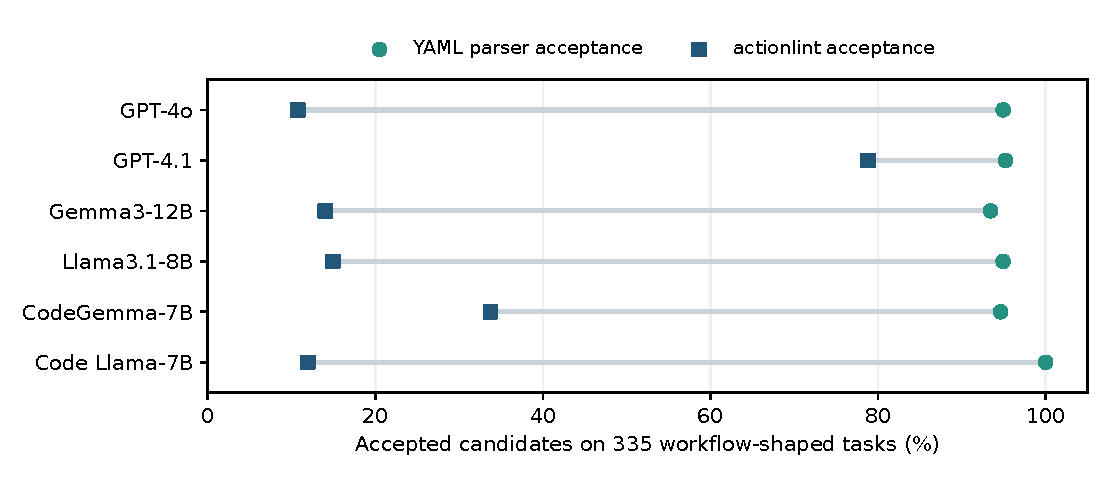
\includegraphics[width=\linewidth]{figures/workflow_validation.pdf}
\caption{Parser and actionlint acceptance of each model on the same 335 workflow-shaped examples. The domain checker tests constraints that a generic YAML loader does not enforce.}
\label{fig:workflow}
\end{figure}

GPT-4o receives a missing-\texttt{on} diagnostic on 237 tasks and action-usage diagnostics on 192 tasks; these categories overlap. Other diagnoses concern obsolete action runtimes, runner labels, expressions, and workflow-specific fields. Under identifier 28, for example, GPT-4o emits a jobs mapping without the workflow trigger; fallback selects the checker-accepted GPT-4.1 candidate. Under identifier 42, GPT-4.1 uses a malformed local-action path and fallback reaches CodeGemma.

The domain result is conditional on the pinned checker and available context. Among the 43 rejected references, 21 have syntax-check diagnoses and 14 have runner-label diagnoses, with possible category overlap. Custom runners, local actions, and reusable workflows can depend on missing repository context. The three audit cases in Appendix~\ref{app:cases} link the numerical results to specific source strings and checker messages.

\begin{table}[H]
\centering\small
\caption{Static acceptance under fixed candidate prefixes and alternative weighting.}
\label{tab:workflowrobustness}
\begin{tabular}{@{}lrrrrr@{}}
\toprule
Candidate pool & Accepted & Row (\%) & Pair (\%) & Page (\%) & Checks\\
\midrule
GPT-4.1 alone & 264 & 78.81 & 81.95 & 79.70 & 1.00\\
First archived candidate & 36 & 10.75 & 11.14 & 4.88 & 1.00\\
First 2 archived candidates & 266 & 79.40 & 82.52 & 79.81 & 1.89\\
First 3 archived candidates & 271 & 80.90 & 84.24 & 81.69 & 2.10\\
First 4 archived candidates & 272 & 81.19 & 84.81 & 82.48 & 2.29\\
First 5 archived candidates & 284 & 84.78 & 85.81 & 86.51 & 2.48\\
First 6 archived candidates & 284 & 84.78 & 85.81 & 86.51 & 2.63\\
\bottomrule
\end{tabular}
\par\vspace{0.3em}{\footnotesize The same 335 rows contain 175 exact description--reference pairs and 127 source pages. Pair and page columns average within each unit before averaging units. Prefixes follow the fixed model priority; checks count sequential static evaluations until acceptance or exhaustion. They do not estimate model calls, latency, or cost.}
\end{table}


The gain over GPT-4.1 remains under the alternative weighting schemes (Table~\ref{tab:workflowrobustness}): 3.86 percentage points per exact task pair and 6.81 per source page, compared with 5.97 per row. The row-weighted paired URL-cluster interval is [3.93, 8.29] percentage points, based on 127 source pages. This describes complementary accepted outputs in the archive. Because the fallback pool contains GPT-4.1, it cannot lose an accepted GPT-4.1 case under the same checker; the 20 additional accepted cases are therefore a coverage result, not evidence of superior inference at equal cost.

The first two candidates already cover 266 tasks. Adding Gemma3, Llama3.1, and CodeGemma raises coverage to 271, 272, and 284; adding Code Llama leaves it at 284. The mean number of sequential static checks is 2.63 for the six-candidate policy. That count excludes generation and does not justify a claim about latency or monetary savings. It shows where the archived coverage increment comes from and why a future equal-budget comparison is necessary.

\subsubsection{Selection framework and implementation boundary}
Figure~\ref{fig:framework} presents the selection stages, and Table~\ref{tab:framework} records their implementation status. The interface in \texttt{select\_configuration.py} accepts candidate files in priority order, returns the selected YAML, and records the attempted candidates and diagnostic decisions. The static stages are evaluated here; execution and human intent review remain subsequent stages.

\begin{figure}[H]
\centering
\begin{tikzpicture}[node distance=0.45cm,box/.style={draw=Accent,rounded corners=2pt,fill=Accent!4,text width=12.5cm,align=left,inner sep=7pt,font=\small},arr/.style={-{Stealth[length=2mm]},color=Accent}]
\node[box] (a) {\textbf{1. Specify task and scope}\quad Record required behavior; distinguish a workflow from a fragment.};
\node[box,below=of a] (b) {\textbf{2. Preserve evidence and obtain candidates}\quad Keep source text, model identity, and transformations.};
\node[box,below=of b] (c) {\textbf{3. Parse each candidate}\quad Record loading failures and empty documents; retain eligible candidates.};
\node[box,below=of c] (d) {\textbf{4. Check scope and select}\quad For workflows, apply actionlint; return a passing candidate or abstain.};
\node[box,below=of d] (e) {\textbf{5. Validate intent and behavior (future)}\quad Use requirement assertions, isolated runs, and review.};
\node[box,below=of e] (f) {\textbf{6. Report outcomes and revise}\quad Separate coverage, similarity, functional success, cost, and failures.};
\draw[arr] (a)--(b);\draw[arr] (b)--(c);\draw[arr] (c)--(d);\draw[arr] (d)--(e);\draw[arr] (e)--(f);
\end{tikzpicture}
\caption{Implemented static-selection framework and its proposed behavioral-validation extension. Evidence preservation, parsing, selection, actionlint checks, and reporting are evaluated on archived candidates; generation and execution are outside the experiment.}
\label{fig:framework}
\end{figure}

\begin{table}[H]
\centering\small
\caption{Implementation boundary of the framework. An accepted parser result is an intermediate state, not an approval for deployment.}
\label{tab:framework}
\begin{tabularx}{\linewidth}{@{}lYY@{}}
\toprule
Stage & This study & Required next evidence\\
\midrule
Task and reference integrity & IDs, hashes, repetition and transformation audit & Independently reviewed task scope and expected behavior\\
Candidate acquisition & Six archived candidates per example & New controlled generation with pinned settings\\
Parser gate and fallback & Implemented and evaluated offline & Broader cases and comparison of fallback orders\\
Domain constraints & actionlint implemented & Repository context and requirement assertions\\
Intent, execution and review & Future extension & Isolated runs, behavioral tests, human judgments\\
Outcome reporting & Implemented for scores and acceptance & Runtime, cost, repair effort and functional success\\
\bottomrule
\end{tabularx}
\end{table}

For a complete-workflow task, the command-line implementation applies the same pinned checks as the experiment and abstains if none of the supplied candidates passes. For fragments it applies the declared parser gate; prospective domain checking would require a fragment-specific schema or a controlled harness. The structural selectors provide separately evaluated exploratory alternatives when reference overlap is the target. Subsequent behavioral validation should compare matched tasks and candidate budgets using functional success and total cost.

\section{Limitations}
Feature identity does not establish YAML semantic equivalence, and a checker-accepted workflow may still omit required behavior, rely on unavailable secrets, or fail at runtime. The original paper's approximately 3\% perfect-match statement lacks a sufficiently explicit definition for us to reproduce that percentage identically. Its 90-case qualitative analysis remains prior work; this extension does not claim new expert labels or inter-rater agreement.

The new lexical and structural scores are independently calculated, while the original embedding and tree-distance columns are reused. Raw-text preprocessing, reference versions, and score definitions differ between the archived and new experiments; comparisons across those variants are descriptive. The documented default for \texttt{all-MiniLM-L6-v2} truncates inputs beyond 256 WordPieces~\cite{sbert}; the released script does not override the sequence-length setting. Long YAML documents may therefore be represented only in part. We cannot recover a historical truncation rate from the stored scores. The structural representation preserves scalar spelling but does not fully model tags on nonempty containers or mapping keys, merge semantics, expression evaluation, or command behavior.

Repeated documentation tasks affect statistical independence. Pair balancing and URL clustering provide sensitivity checks, but exact matching misses paraphrases and duplicated tasks can cross page boundaries. The selector rules use no reference answer, but the policy comparison, root-removal check, and workflow robustness analysis all use the same released dataset. They are exploratory analyses, not independent confirmation. A holdout evaluation is needed before generalizing selection performance.

The workflow comparison is conditional on the 335 shape-defined tasks and actionlint 1.7.7 with external integrations disabled. Custom runner labels and repository-local dependencies can produce diagnoses that require unavailable context; conversely, a zero-diagnostic result cannot establish that remote actions or services exist or behave as intended. The 2025 checker reduces temporal drift but cannot reconstruct the authors' exact environment. Fallback can inspect up to six distinct archived responses, whereas the individual-model baseline supplies one. The measured coverage gain therefore uses a larger candidate pool; inference cost, generation latency, and equal-budget repeated sampling were not measured.

External validity is limited to documentation-derived tasks, six historical model labels, and GitHub Actions. Public documentation may have appeared in training data. Model size, training, and hosting differ, so the results do not identify a causal effect of code specialization.

\section{Implication of Research in Other Areas}
The workflow results identify a useful boundary for other configuration-generation tasks: a generic parser can accept a document that omits a field required by the target system. In this dataset, syntax fallback accepts all 335 workflow tasks, but only 43 selected outputs pass the workflow checker. Infrastructure manifests or container definitions would need the corresponding domain checks before parser acceptance could serve as a useful quality gate. Their actual benefit cannot be inferred from the GitHub Actions counts.

The evaluation lesson also applies to benchmark design. Giving each documentation row equal weight, giving each task pair equal weight, and giving each page equal weight produce different comparisons. A benchmark for another software engineering task should state which of those units matches its intended use. For a developer-facing selector, the 51 abstentions are equally consequential: they identify cases requiring another candidate or review. Whether this behavior reduces repair effort is the next empirical question.

\section{Future Work}
The next experiment should test whether the observed static gains survive new tasks and equal candidate budgets. Tasks should be collected independently and split by source page and near-duplicate family before policy choice. Single-model repeated sampling, multi-model fallback, and consensus should receive the same candidate or inference budget. Functional success, checker acceptance, total cost, and reviewer effort should be reported separately, with uncertainty at the task-cluster level.

Execution-based evaluation needs repository fixtures and explicit requirement assertions. Complete workflows should run in an isolated environment; fragments need a harness defined before generation. Independent reviewers could assess omissions, additions, and intent mismatches while reporting disagreements. Domain checks, consensus selection, and bounded diagnostic repair should also be combined in an ablation study: this paper evaluates their static and overlap outcomes separately, so the best way to combine them remains an empirical question.

A further replication could recompute the archived embedding and tree-distance measures from preserved inputs, contrasting the released preprocessing with parser-aware alternatives.

\section{Conclusions}
The released dataset does not support a single overall model ranking. GPT-4o leads on archived row-level cosine similarity, but its paired difference from GPT-4.1 is not significant. Page-balanced weighting reverses their order, and GPT-4.1 passes the workflow checker much more often. RQ1 and RQ2 thus identify measurement and aggregation choices that change the comparison.

For RQ3, consensus improves leaf-only structural agreement from 0.116 to 0.127 with a positive URL-cluster interval, while reducing lexical agreement. Checker-guided fallback accepts 284 of 335 workflow-shaped tasks versus 264 for GPT-4.1 and abstains on 51. The reference audit exposes perfect tree scores caused by failed parses, and the root-feature ablation separates persistent consensus gains from representation-dependent minimality gains. These findings concern the archived candidate pool; functional correctness requires behavioral evaluation.
